\begingroup
\begin{minipage}{\linewidth}
\raggedright
\subsection{Plotting with Matplotlib (Python)}
Install with \texttt{python3 -m pip install matplotlib}, then run
\texttt{python3 MatplotlibExample.py}. Supply equally sized lists
of $x$ and $y$ values; \texttt{plot} connects points in list order.
\texttt{subplots} creates the figure and its plotting area.
\lstinputlisting[style=C++,language=Python,showstringspaces=false]{../compile/MatplotlibExample.py}
\begin{center}
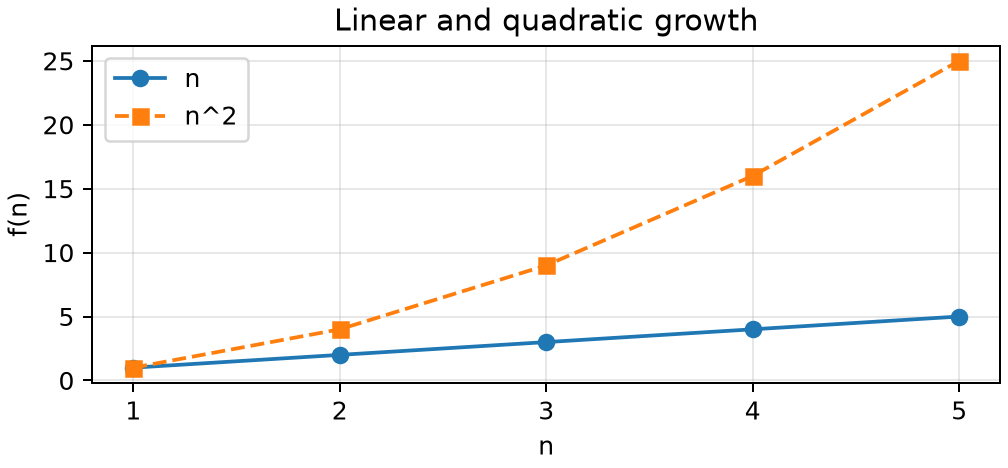
\includegraphics[width=0.88\linewidth]{../compile/matplotlib_example.png}
\end{center}
\textbf{Other plot types.} Replace a \texttt{plot} call with
\texttt{ax.scatter(x, y)} for unconnected points or
\texttt{ax.bar(x, y)} for bars. \texttt{label} names a series;
\texttt{legend()} displays those names. \texttt{fig.savefig("graph.pdf")}
exports a vector PDF. Close saved figures with \texttt{plt.close(fig)}
when generating many plots.
\href{https://matplotlib.org/stable/users/explain/quick_start.html}{Official Matplotlib quick start.}
\end{minipage}
\par
\endgroup
